\section{Optimization of the telluric correction}
\label{sec:configuretion_overview}

\subsection{Selection of most appropriate calibrations}

The EDPS workflows allow to express a preference w.r.t. the
calibrations to be associated, e.g. raw calibrations or master
calibrations (pre-computed from previous runs).

This is done by setting the Calibration Preference in the Raw Data
tab.

In the case of the molecfit workflow, there are no master calibrations
available at the moment, therefore this option is not supported.

\subsection{Adjusting the recipe parameters {\it before } fitting}
\label{sec:adjust_recipe_parameters}

Recipe parameters can be configured per dataset from the configuration
editor (Section \ref{sec:configuration_editor}. If no action is taken,
default recipe parameters (either recipe defaults or automatically set
by the workflow depending on the type of input data) are
used. Defaults can be changed before starting the reduction, or
after (in this case, a new configuration is created).

In the case of \pipename\ the fit step carried on by the task {\bf
  atmospheric\_model} takes a lot of time: adjusting recipe parametes
{\it after} each recipe execution is indeed inefficient.

The \pipename\ EDPS workflow offers the possibility to inspect the
recipe parameters {\it before} fitting the reference spectrum. This is
particularly relevant for those parameters that can be assessed after
a visual inspection of the spectrum to fit (e.g., wavelength range to
consider, molecules to include in the fit, degree of the polynomial
continuum).

To do so, follow this procedure:

\begin{itemize}

\item Open the configuration editor (Section
  \ref{sec:configuration_editor}) for the desired
  dataset/configuration in the Reduction Queue and set the workflow
  parameter {\bf set\_parameters\_only} has to be set to {\bf true} {\it
    before starting the reduction}. This can be done also from the Raw
  Data tab {\it before} creating the datasets.

\item Select the datasets (those with {\bf
  set\_parameters\_only = 'true'}) and start the reduction by pressing
  the Reduce button in the Reduction Queue.

\item The reduction will start. The task {\bf
  parameter\_configuration} automatically set the recipe parameter,
  which are passed to the next tasks. The next tasks do not execute
  any recipe and do not produce any output, but are automatically set
  to {\tt COMPLETED}. They are associated to a recipe named {\tt
    skip\_execution}.

\item Open the configuration editor (Section
  \ref{sec:configuration_editor}), select the task {\bf
    parameter\_configuration} and edit the parameters according to the
  needs. Visual inspection of the data might help in deciding the
  most appropriate values. To visually inspect the data, press on
  the magnifying lens symbol close to the {\bf parameter\_configuration}
  task (see Section \ref{sec:quality_plots}).


\item Once the new parameter are set, save the new configuration. The
  reduction of the new configuration can be started. Once the
  parameters have been optimized, save a new configuration with {\bf
    set\_parameters\_only = 'false'} and start the reduction.  The
  following tasks will now perform the fit, compute the atmospheric
  transmission, and correct the science spectrum with the correct
  recipes.

\item If final results are still not satisfactory and recipe
  parameters have to be modified again, create a new configuration
  with {\bf set\_parameters\_only = 'true'} and repeat the process.


\end{itemize}

\subsection{Tipps on how to set parameters}

The most common recipe parameters that might need to be adjusted, even
after the automatic setting done in the workflow, are:

\begin{itemize}

\item {\tt WAVE\_INCLUDE}. A list of wavelength values in micron,
  comma separated, that specifies the boundaries of the wavelength
  regions to include in the fit. Try to select short regions that contain
  clear and intense absoprtion lines. Avoid lines close to
  saturation. Leave a few pixels outside the lines to facilitate the
  determination of the continuum level.  Please, not that a continuum
  level is computed for each region. The more and broade wavelength
  regions are defined, the longer the fit will be, and it is not
  guarantee that the fit will be better than one obtained with less
  numerous and narrower regions.

\item {\tt WAVE\_EXCLUDE}. A list of wavelength values in micron,
  comma separated, that specifies the boundaries of the wavelength
  regions to exclude in the fit. An exclusion region inside an
  inclusion region does not divide the inclusion region in 2 smaller
  regions: a single continuum level is still computed for that
  inclusion region.

\item {\tt LIST\_MOLEC}, {\tt FIT\_MOLEC}, {\tt REL\_COL}. The first
  parameter, {\tt LIST\_MOLEC}, contains the comma-separated list of
  molecules to include in the fit. Be sure to include only molecules
  that have a significant impact within the visible spectral
  region. Each individual molecule can be fit (the corresponding temr
  in {\tt FIT\_MOLEC} is 1) or computed (the corresponding term in
  FIT\_MOLEC is 0) considering typical abundance ratios and relative
  column densities (the corresponding value in {\tt REL\_COL} is
  used). Note that the number of elements in FIT\_MOLEC and {\tt
    REL\_COL} must be the same as the number of elements in {\tt
    LIST\_MOLEC}.
  
\item {\tt CONTINUUM\_N} The polynomial degree to fit the continuum. A
  comma separated list of values can be provided, each per every
  wavelegth region defined in {\tt WAVE\_INCLUDE}.

\item {\tt WLC\_N}. The polynomial degree to fit the wavelength
  adjustment. A global wavelength solution is used for all the
  specgtral range. It is recommended to leave it to 1, unless telluric
  features are fitted all over the spectrum, including the edges, to
  avoud interpolation and extrapolation effects.
  
  
\item {\tt FIT\_RES\_BOX}, {\tt FIT\_RES\_LORENTZ}, {\tt RES\_BOX},
  {\tt RES\_LORENTZ}, {\tt VARKERN}. These are parameters that specify
  the shape of the line profile (line spread function). For wide slits
  where the box-car contribution is relevant, set {\tt FIT\_RES\_BOX =
    1} and {\tt RES\_BOX} different from 0. If the box-car
  contribution does not have to be included, then set both {\tt
    FIT\_RES\_BOX} and {\tt RES\_BOX} to 0.  {\tt VARKERN} has to be
  set to:
  \begin{itemize}
  \item {\tt VARKERN = 'TRUE'} if the resolving power ($\lambda/$fwhm) is constant
    with wavelength.
    \item {\tt VARKERN = 'FALSE'} if the spectral resolution (fwhm) is constant with wavelength.
  \end{itemize}
\end{itemize}



\subsection{Configuration of parameters: the configuration editor}
\label{sec:configuration_editor}
The data reduction of each dataset can be configured according to the scientific needs using an appropriate configuration editor.


The \edps\ workflows contain two types of parameters and they both
have default values that can be modified to improve the data
reduction.
\begin{itemize}

\item {\bf Workflow parameters} (for some workflows only) are global and they are applied to the entire workflow. They are accessible both in the `Raw Data`
tab, prior to the creation og a dataset, and in the `Reduction
Configuration` editor, in the `Reduction queue` tab.  Note: some
workflow parameters were already configured before creating the
dataset and sending it to the reduction queue.  Here, they can be
changed again. Please, note that the parameters have an effect only on
the files that are already in the dataset.  If one specifies a
parameter that should include extra files in the dataset (e.g., the
inclusion of more calibrations), files are not added and the reduction
might fail.  If you need to change a parameter that modifies the
dataset content, please go back to the Raw data tab and create a new
dataset.

\item {\bf Recipe parameters} are specific to the individual recipes and can be configured per task. They are accessible in the `Reduction Configuration` editor, in the `Reduction queue` tab.

\end{itemize}

This editor allows to configure the data reduction for a given dataset
by specifying workflow and recipe parameters.



Note: some workflow parameters were already configured before creating the dataset and sending it to the reduction queue.
Here, they can be changed again. Please, note that the parameters have an effect only on the files that are already in the dataset. 
If one specifies a parameter that should include extra files in the dataset (e.g., the inclusion of more calibrations), files are not added and the reduction might fail. 
If you need to change a parameter that modifies the dataset content, please go back to the Raw data tab and create a new dataset.





To open the editor, click on
the wheel button 
\includegraphics[width=0.8cm]{../common/figures/configure_dataset.jpg} next to the dataset you desire to configure the reduction for. A window with the
configuration editor appears as shown Figure \ref{fig:configuration_editor_0}.


\begin{figure}[h!]
\centering
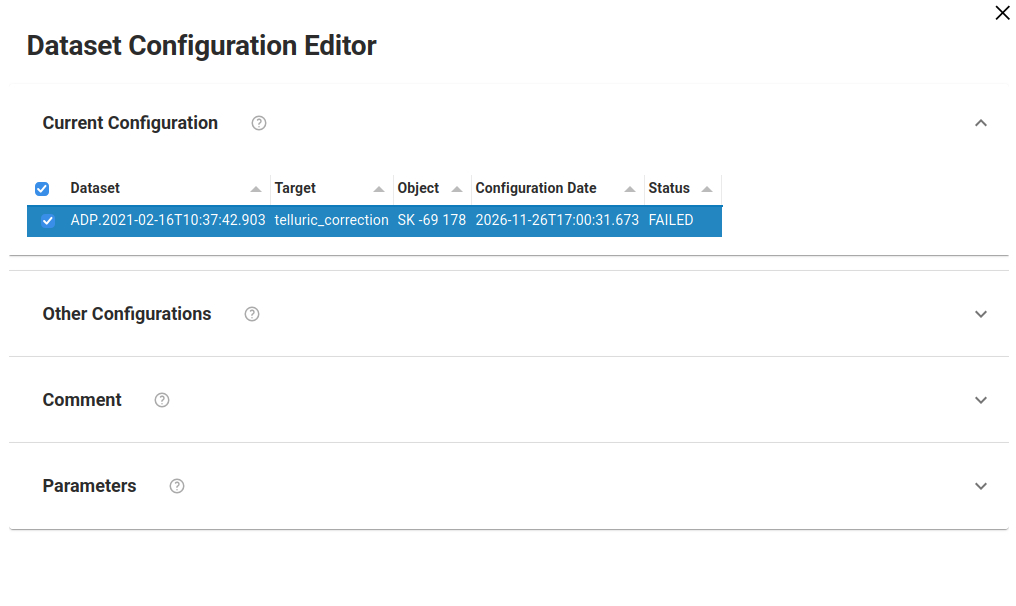
\includegraphics[width=0.9\textwidth]{../instrument_tutorial/figures/configuration_editor_0.jpg}
\caption{The Reduction Configuration editor. It contains 4 sections, that indicate the current configuration, list of other configurations to set, comments to insert, and the parameters to modify.}
\label{fig:configuration_editor_0}
\end{figure}



The editor is divided into 4 parts, which can be accessed pressing the corresponding expansion arrow. 
\begin{itemize}

\item {\bf Current configuration.} It indicates the name of the selected configuration for a given dataset (Figure \ref{fig:configuration_editor_1}).

\item {\bf Other configurations.} It allows to specify other configurations, to which the changes shall be copied to (Figure \ref{fig:configuration_editor_2}.

\item {\bf Comment} It allows to specify a comment to describe the configuration. It is possible to append or replace a comment (Figure \ref{fig:configuration_editor_3}).
Comments can be changed on all configurations. It is possible to save the comment for the current configuration only, or for all
the selected configurations.

\item {\bf Parameters.} A window as in Figure \ref{fig:configuration_editor_4} appears.

The window allows to: 
\begin{itemize}

\item Select the parameter set. A pre-determined list of workflow parameters and recipe parameters for a given 
  use case. For the majority of the cases, the "science" parameter set can be used.

\item Edit the workflow parameters. These are parameters that regulates the reduction strategy, e.g. whether to 
  use a given calibration or not, or to trigger a certain reduction step. Note that if the changes imply that 
  some files not in the dataset are needed, the reduction might fail. In case, go back to the raw data tab, edit the 
  workflow parameters there, and recreate the datasets.

\item Edit the recipe parameters. These are parameters associated to the recipe of a given task. 
  Note: the same recipe parameters can be configured differently for the tasks that run the same recipe.
  Default parameters are shown (albeit some parameters can be dynamic, e.g. `EDPS` changes
  their value depending on the type of input data).  
\end{itemize}

Change the values according to the needs and then select whether to save it to the current or the selected configurations. 
Note, complete configurations cannot be modified, new configurations will be automatically created instead.



\end{itemize}

\begin{figure}[h!]
\centering
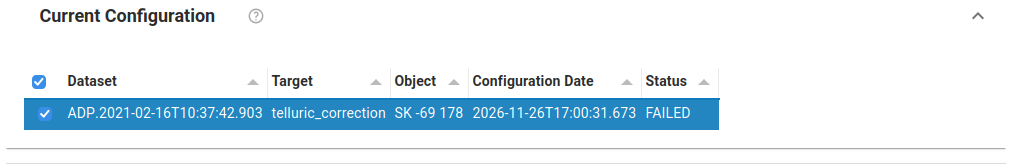
\includegraphics[width=0.9\textwidth]{../instrument_tutorial/figures/configuration_editor_1.jpg}
\caption{The first part of the Reduction Configuration Editor, that indicates the selected configuration.}
\label{fig:configuration_editor_1}
\end{figure}
 

\begin{figure}[h!]
\centering
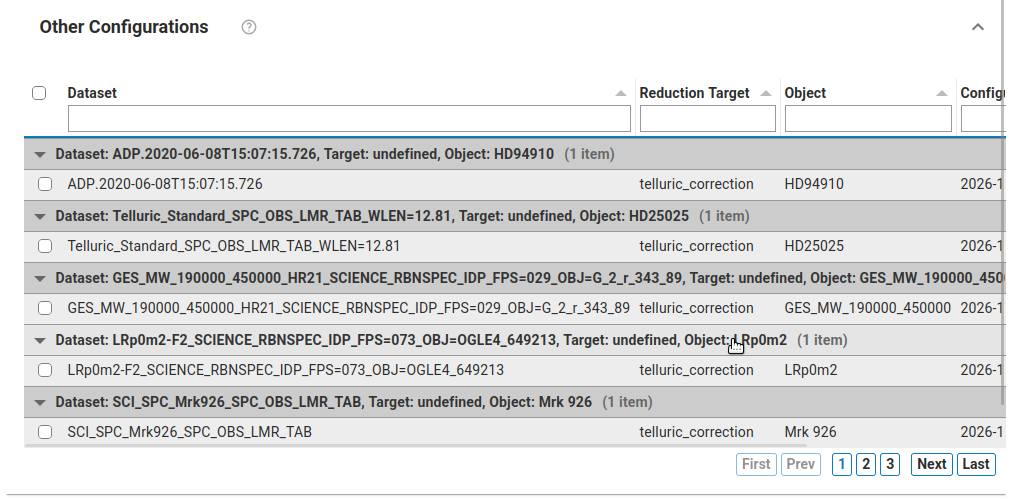
\includegraphics[width=0.9\textwidth]{../instrument_tutorial/figures/configuration_editor_2.jpg}
\caption{The second part of the Reduction Configuration Editor, that indicates other configurations for which we'd like to apply the changes.}
\label{fig:configuration_editor_2}
\end{figure}


\begin{figure}[h!]
\centering
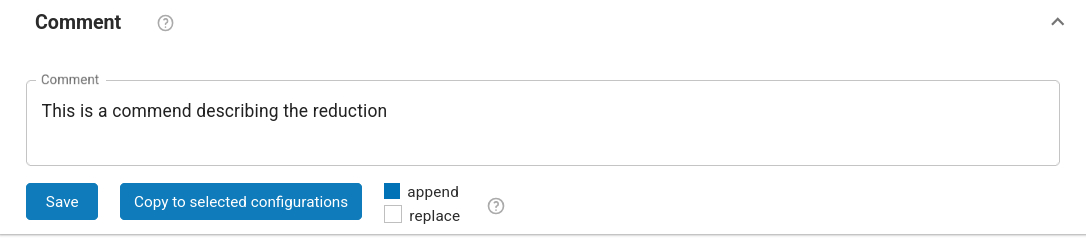
\includegraphics[width=0.9\textwidth]{../instrument_tutorial/figures/configuration_editor_3.jpg}
\caption{The third part of the Reduction Configuration Editor, that allows to specify a comment to the selected configurations.}
\label{fig:configuration_editor_3}
\end{figure}


\begin{figure}[h!]
\centering
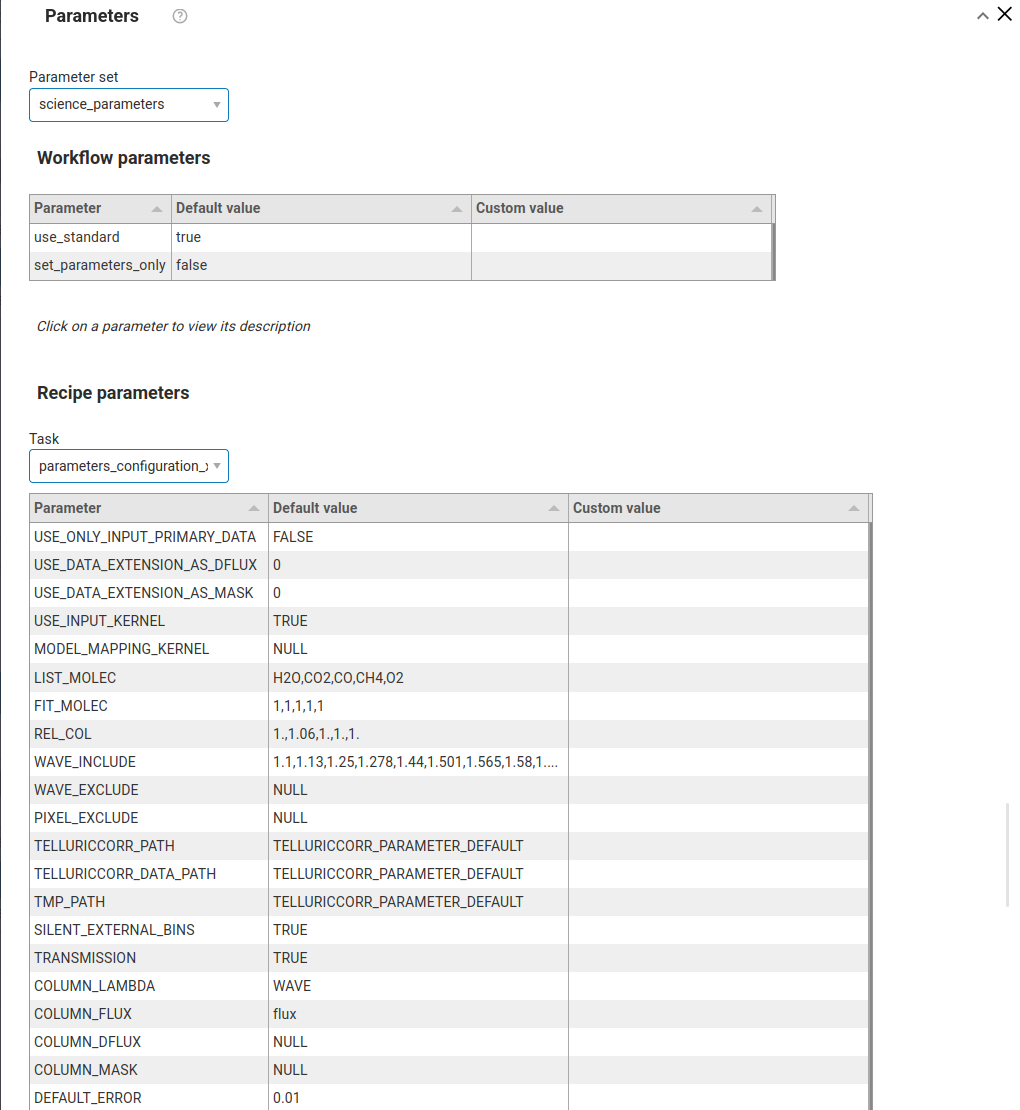
\includegraphics[width=0.9\textwidth]{../instrument_tutorial/figures/configuration_editor_4.jpg}
\caption{The fourth part of the Reduction Configuration Editor, that allows to specify the parameters sets and the recipe parameter per task. These settings can be applied to the "Selected Configuration" (Fig. \ref{fig:configuration_editor_1}) or to the "Other Configurations (Fig. \ref{fig:configuration_editor_2}). }
\label{fig:configuration_editor_4}
\end{figure}






